\section{Spectral element method on non conforming meshes}
Equation \ref{eq:weakform} is the problem we will be attempting to solve. However, the equation must still hold for every function $v \in H_0^1(\Omega)$. This section presents the method used for the discretization of the problem, namely the spectral element method on a non conforming mesh. 

The first part of the task is the discretization of the domain $\Omega$. As explained in the introduction, we will use non conforming meshes. So we will present such meshes, present their particularities and explain how we will handle them.   

The second part of the task is the discretization of equation \ref{eq:weakform}. The method here presented is the spectral element method, which consists of using high degree piece-wise polynomials as basis functions. We will first show how to obtain the linear system of equation ($Au=b$) that arises with this method. We will afterwards present the one dimensional basis functions used and the location of the nodes on the 1D reference element. We will then explain how to construct the global basis functions in the presence of hanging nodes. We will finally show how to compute the right hand side of the linear system and how to perform an efficient matrix-vector product without having to explicitly construct the matrix $A$.

\subsection{Discretization of the domain}

Let us first tackle the discretization of the domain. In classical AMR, the mesh depends on the problem to solve and the refinement is performed to obtain the fact that the error committed on each quadrant is roughly the same (see \cite{amrError}). But that is not the focus of the work done here. Instead, let us assume that we already have a mesh $G$ consisting of unstructured quadrilaterals (denoted $\Omega_e$) and that might be non conforming, i.e. where we have the presence of hanging nodes. As always, we have : 

\begin{align*}
G &= \bigcup\limits_{e} \Omega_e\\
\Omega_i \cap \Omega_j &= \emptyset &\text{if $i\neq j$}
\end{align*}

\begin{figure}
\centering
\includegraphics[scale=0.45]{Theory/hang_ex.png}
\caption{Example of a legal non conforming mesh (it is 1-irregular). We can see that we have two hanging nodes in red since they are not vertices of the bigger quadrants neighboring them.}
\label{hang_ex}
\end{figure}

We can define a hanging node as being a node that is not shared between all its neighboring quadrants. We can note that hanging nodes can only be found on edges. Figure \ref{hang_ex} shows an example of a mesh containing hanging nodes. We can see that the vertices in red are hanging nodes since they are vertices of the smaller quadrants neighboring them but not of the bigger quadrants neighboring them. Those nodes will require a special treatment in the spectral element method. 

\begin{figure}
\centering
\includegraphics[scale=0.45]{Theory/hang_illegal.png}
\caption{Example of an illegal non conforming mesh (it is 2-irregular). We can see that the top left quadrant has four neighbors through its south edge while we imposed a maximum of two. }
\label{hang_illegal}
\end{figure}

We have however one restriction to make on the mesh. We will allow two neighboring quadrants to have only one level of difference in the refinement. This means that the number of neighbors of a quadrant through a given edge is maximum two. We call such meshes 1-irregular. Figure \ref{hang_illegal} shows an example of an illegal non conforming mesh. We can see that on that mesh the top left quadrant has four neighbors through its south edge. Since the maximum difference of the levels of refinement between two neighboring quadrants is two, such a mesh is called 2-irregular.  Handling all possibilities of hanging faces for a general $k$-irregular mesh (with $k>1$) is impossible and that is why we (and the vast majority of others) consider as illegal meshes such as the one presented in figure \ref{hang_illegal}.

For the rest of this chapter, it is important to note that, in a 1-irregular mesh, a hanging edge (an edge containing hanging nodes) is always half of a non hanging edge for its neighboring quadrant.

Once we have our mesh, it is clear that we can compute the integral of any scalar function $g$ as the sum of integrals on the quadrants. Formally, we have :  

\begin{align}
\int_\Omega g\:dxdy = \sum_e \int_{\Omega_e} g\:dxdy \label{eq:int}
\end{align}

All the integrals we compute will be performed quadrant by quadrant and then summed. 

\subsection{Discretization of equation \ref{eq:weakform}}

Since equation \ref{eq:weakform} must hold for every function $v \in H_0^1(\Omega)$, it is not very practical. We will therefore restrict ourselves to $V^h \subset H_0^1(\Omega)$, where $V^h$ has a finite dimension. Let us denote the functions that form the basis of $V^h$ by $\phi_1,..., \phi_N$ (therefore, the space $V^h$ is of dimension $N$). We will define explicitly those basis functions later. 

Using Galerkin approximation, we will also restrict our search of the solution to $V^h$. Let us denote this solution $u^h$. Therefore, we have that : 

$$u^h = \sum_{j=1}^N u_j \phi_j $$

Asking equation \ref{eq:weakform} to be satisfied for every function in $V^h$ is equivalent to ask it to be satisfied for every function of its basis. As a result, the discretized version of equation \ref{eq:weakform} is given by : 

\begin{align}
\sum_{j = 1}^N \int_\Omega \nabla \phi_i \cdot \nabla \phi_j \:dxdy \: u_j &= -\int_\Omega f\phi_i \:dxdy &\text{for $i=1,...,N$} 
\end{align}

Solving this to get the nodal values $u_j$ is actually solving a linear system of equations $\textbf{Au}=\textbf{b}$ where we define : 

\begin{align}
A_{ij} &= \int_\Omega \nabla \phi_i \cdot \nabla \phi_j \:dxdy \label{eq:A}\\
b_i &= -\int_\Omega f\phi_i \:dxdy \label{eq:b}
\end{align}

Those integral will be performed using equation \ref{eq:int}.

\subsection{Basis functions on the reference element and Gauss-Lobatto-Legendre nodes}

As shows equations \ref{eq:A} and \ref{eq:b}, we need to compute integrals to solve the problem. Here, we will perform the integration using Gauss-Lobatto-Legendre (GLL) quadrature. The particularity of 1D GLL nodes is that they include the end points of the interval on which we compute the integral. For example, on the one dimensional reference element, it means that the GLL nodes include $\xi = -1$ and $\xi=1$. This particularity enables us to use the GLL nodes both as quadrature points and as global nodes where we compute our numerical solution. We will see later that this allows us to compute the matrix-vector product very efficiently. 

For $p+1$ GLL nodes, the quadrature integrate exactly polynomials of degree at most $2p-1$. It is less than for the Gauss-Legendre quadrature (which achieve to integrate exactly polynomials up to order $2p+1$). The way to compute the GLL nodes and their weights is for example detailled in \cite{gll_nodes}. Table \ref{gll_values} shows the values for different degrees. We can see that the nodes are not uniformly distributed but they tend to cluster near the end points $\xi = -1$ and $\xi=1$.

\begin{table}
\centering
\begin{tabular}{c|cc}
\hline
 Number of nodes $p+1$ & Points $\xi_i$ & Weights $w_i$\\
 \hline
 2 & $\pm 1$ & $1$ \\
 \hline
 3 & $\pm 1$ & $\frac{1}{3}$\\
    & 0			   & $\frac{4}{3}$\\
 \hline
 4 & $\pm 1$ & $\frac{1}{6}$\\
    & $\pm \sqrt{\frac{1}{5}}$  & $\frac{5}{6}$\\
\hline
5 & $\pm 1$ & $\frac{1}{10}$\\
   & $\pm \sqrt{\frac{3}{7}}$ & $\frac{49}{90}$\\
   & $0$ & $\frac{32}{45}$\\
   \hline
\end{tabular}
\caption{Values of the GLL nodes and the associated weights on the reference one dimensional element for the first few degrees.}
\label{gll_values}
\end{table}

Let us denote the $p+1$ GLL nodes on the reference 1D element by $\xi_0$, $\xi_1$, ..., $\xi_p$. Since the GLL nodes contain the end points of the interval, we can also use them as global nodes. We will use Lagrangian polynomials for the interpolation. Let us denote them $l_0(\xi)$, $l_1(\xi)$, ... , $l_p(\xi)$. Let us recall that : 

$$ l_i(\xi) = \prod_{j=0 , j\neq i}^p \frac{\xi - \xi_j}{\xi_i  - \xi_j}$$

For the following parts of this chapter, it is very important to note that :

$$ l_i(\xi_j) = \delta_{ij} $$ 

Where $\delta_{ij}$ is to be understood as the Kronecker delta. This fact will allow us later to compute the matrix-vector product in a very efficient way. 

Let us also use this opportunity to define the derivation matrix $H$ as : 

\begin{align}
H_{ij} = l_i'(\xi_j) \label{eq:derivation_matrix}
\end{align}

Let us now define the basis functions on the 2D reference element. In 2D, we will use $(p+1)^2$ nodes, tensor product of the 1D GLL nodes. If we denote the 1D GLL nodes by $\xi_i^1$, the 2D nodes are thus located at :

\begin{align*}
(\xi_i, \eta_j) &= (\xi^1_i,\xi^1_j) &\text{for $i,j=0,1,...,p$}
\end{align*}

On the reference quadrant $\xi, \eta \in [-1;1]$, we have in the same way that the basis function associated with node $I$ located at $(\xi_i,\eta_j)$ is given the tensor product of the 1D basis functions : 

$$\phi_I(\xi,\eta) = l_i(\xi)l_j(\eta)$$

Thus, if we want to obtain the value of a field $u$ in the reference quadrant, whose value at node $I$ is given by $u_{ij}$, we interpolate as : 

\begin{align*}
u(\xi,\eta) = \sum_{i=0}^p\sum_{j=0}^p u_{ij}l_i(\xi)l_j(\eta)
\end{align*}

\subsection{Global basis function}

Let us first mention the distinction between global and local nodes. Each quadrant has $(p+1)^2$ local GLL nodes but that does not mean that all of them are global nodes, since some might be hanging. As explained in \cite{hang_treat}, one solution consists to treat hanging nodes as global nodes and then add equations in the linear system $Au=b$ to enforce the continuity of the numerical solution. Another solution is to immediately enforce the continuity of the numerical solution by having continuous global basis function. This is what is done here. We will consider $N$ global nodes (that are the GLL nodes for at least one quadrant) and give them a global unique index $I = 1,...,N$. 

We want our global basis function $\phi_I$ to be a piece-wise polynomial of order $p$ and to have a value of exactly $1$ at global node $I$ and to be equal to $0$ on any other global node. 

In order to define such a function, we first need a mapping that goes from the 2D reference element to the actual quadrant $e$, i.e. $x^e(\xi,\eta)$ and $y^e(\xi,\eta)$ that for quadrant $e$ give the actual coordinates of any point in the reference element. Let us also define the inverse mappings $\xi^e(x,y)$ and $\eta^e(x,y)$. 

The last thing we need is a global to local operator that gives for local node $(\xi_i,\eta_j)$ on quadrant $e$ the weight of global node $I$. Let us denote this operator $R^e_{ij}(I)$. In a conforming mesh, since each local node correspond to a global node, $R^e_{ij}(I)$ can only be equal to 0 or to 1. In a non conforming mesh, however, the value of $R^e_{ij}(I)$ must be computed to ensure the continuity of the global basis function. For example, if we have hanging nodes on the east edge of quadrant $e$ (where $i=p$), then $R^e_{pj}(I)$ is given by : 

\begin{align*}
R^e_{pj}(I) &= l_k \left(\frac{\xi_j}{2}\pm \frac{1}{2}\right) &\text{if $I$ is the $k$-th global node on the non hanging east edge}
\end{align*} 

More explanation about how to compute the operator $R^e_{ij}(I)$ can be found in \cite{hang_handle}. The plus or minus sign in the above formula comes from the fact that a hanging edge can be the first or the second part of the larger non hanging edge. This is why we accept only 1-irregular meshes : because we only have to handle two cases when we compute $R^e_{ij}(I)$. If we accepted $k$-irregular meshes with $k>1$, we would have too many different cases to look at. 

With this operator and our mapping, it is then possible to compute the value of the basis function associated with node $I$ inside any element $e$. It is given by : 

\begin{align}
\phi_I(x,y) &= \sum_{i=0}^p\sum_{j=0}^p R^e_{ij}(I) \: l_i(\xi^e(x,y))\: l_j(\eta^e(x,y)) &\text{if $(x,y) \in \Omega_e$}\label{eq:global_basis}
\end{align}

\begin{figure}
\centering
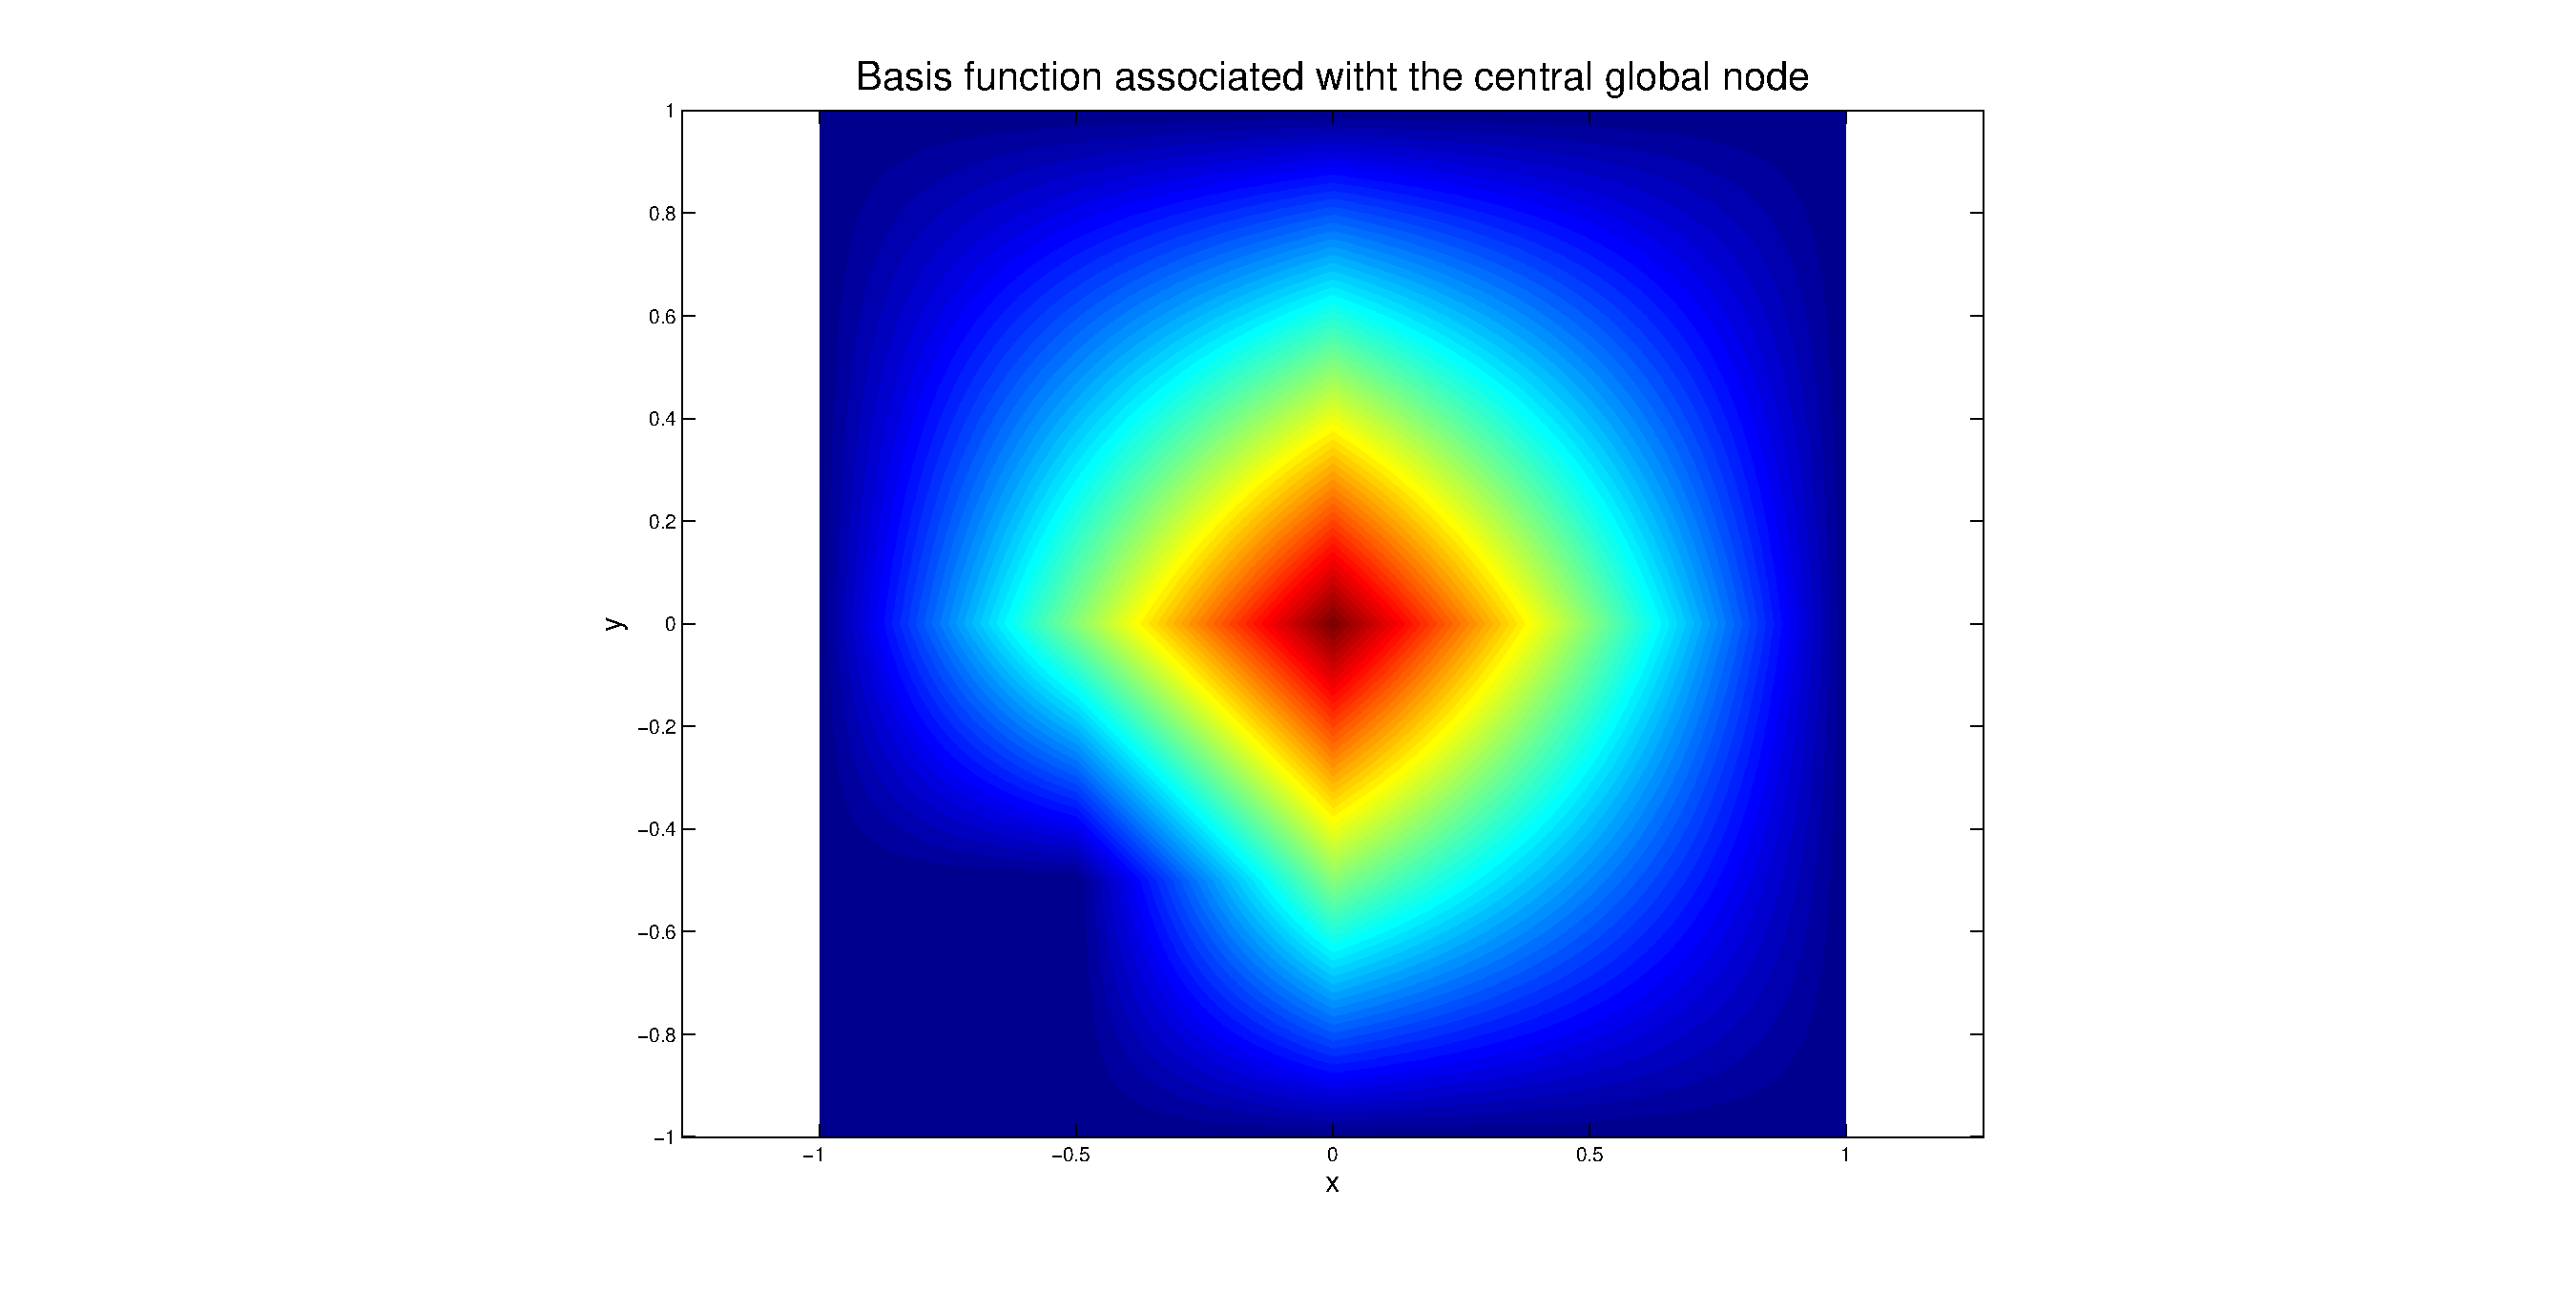
\includegraphics[scale=0.35]{Theory/global_basis_func.eps}
\caption{Global basis function associated with the global GLL node located in the center of the mesh presented in figure \ref{hang_ex} for $p=1$.}
\label{global_basis_func}
\end{figure}


Figure \ref{global_basis_func} shows a global basis function on the mesh presented in figure \ref{hang_ex} for $p=1$. We can see that it is not entirely trivial since the global node associated with the basis function has a influence in quadrants where we have hanging nodes. We can also see that it is indeed a continuous function that is a piece-wise bilinear polynomial. 

Let us also note that there is no global basis function associated with a hanging node. 

In practice, we do not build the operator $R^e_{ij}(I)$ explicitly since only nodes located on edges can be hanging and the p4est library helps us to treat hanging nodes (see the implementation chapter for more details).  

\subsection{Computing the right-hand side}

Now that we have defined our global basis functions, it is possible to perform the integration needed to compute $b_j$ (equation \ref{eq:b}). As explained before, we will perform the integration quadrant by quadrant. Let us denote : 

$$ b_I^e = -\int_{\Omega_e} f\phi_I\:dxdy$$

We obviously have that $b_I = \sum_e b_I^e$. Let us also define the reference element associated with quadrant $e$ by $\hat{\Omega}_e$ and the jacobian of the mapping as : 

$$ J^e (\xi,\eta) = \begin{pmatrix}
\frac{\partial x^e}{\partial \xi} & \frac{\partial x^e}{\partial \eta}\\
\frac{\partial y^e}{\partial \xi} & \frac{\partial y^e}{\partial \eta}
\end{pmatrix}$$

Then the integration on quadrant $e$ becomes : 

$$b_I^e = -\int_{\hat{\Omega}_e} f(x^e(\xi,\eta),y^e(\xi,\eta)) \phi_I(x^e(\xi,\eta),y^e(\xi,\eta)) |J^e(\xi,\eta)| \: d\xi d\eta$$

Using equation \ref{eq:global_basis}, we get : 

$$b_I^e = -\int_{\hat{\Omega}_e} f(x^e(\xi,\eta),y^e(\xi,\eta)) \left( \sum_{i=0}^p\sum_{j=0}^p R^e_{ij}(I) l_i(\xi)l_j(\eta) \right) |J^e(\xi,\eta)| \: d\xi d\eta $$

This is where the fact that our global nodes are also GLL nodes becomes important. To alleviate a little the formulas, let us define two new notations :  $J^e(\xi_m,\eta_n) = J^e_{mn}$ and $f(x^e(\xi_m,\eta_n),y^e(\xi_m,\eta_n)) = f^e_{mn}$. Using the GLL quadrature rule, we have : 

$$ b_I^e = - \sum_{m=0}^p\sum_{n=0}^p w_m w_n f^e_{mn} \left( \sum_{i=0}^p\sum_{j=0}^p R^e_{ij}(I) l_i(\xi_m)l_j(\eta_n) \right) |J^e_{mn}|$$

Since $l_i(\xi_j) = \delta_{ij}$, this becomes : 

$$  b_I^e = - \sum_{m=0}^p\sum_{n=0}^p w_m w_n f^e_{mn} R^e_{mn}(I) |J^e_{mn}|$$

This expression looks more complicated than it actually is. Indeed, the operator $R_{mn}^e(I)$ is often equal to zero. It is non zero only if in quadrant $e$, the local node $(m,n)$ is the global node $I$ (in which case it is equal to 1) or if the local node $(m,n)$ is located on a hanging edge where the global node $I$ has an influence. Therefore, in a quadrant where we do not have hanging nodes, and if the local node $(m,n)$ has $I$ as global number, we simply have : 

$$b_I^e = - w_m w_n f^e_{mn} |J^e_{mn}|$$

\subsection{Computing a matrix-vector product}

As said in the introduction, we will use an iterative method to solve the system presented by equations \ref{eq:A} and \ref{eq:b}, namely the preconditioned conjugate gradients. As a result, we do not need to build the matrix $A$ explicitly but rather we need to be able to perform a matrix-vector product $Au$ where $u$ is a vector containing the values of our numerical solution at the global nodes, i.e. $u_I$ is the value of the solution at global node $I$. By linearity of the integral and the derivative, and the definition of $u^h$, we have : 

\begin{align*}
(Au)_I =& \sum_{J=1}^N \int_\Omega \nabla \phi_I \cdot \nabla \phi_J \:dxdy \: u_J\\
=& \int_\Omega \nabla \phi_I \cdot \nabla\left(\sum_{J=1}^N \phi_Ju_J\right)\:dxdy\\
=& \int_\Omega \nabla \phi_I \cdot \nabla u^h \: dxdy
\end{align*}

Just as in the previous subsection, we will compute this integral quadrant by quadrant. The first thing we want to do is to compute the value of $u^h$ at the local GLL nodes on quadrant $e$. Let us define, $u^e_{mn}$ as this local value : 

$$u^e_{mn} = \sum_{I=1}^N R_{mn}^e(I) u_I$$

Let us then define $u^e$ as the restriction of $u^h$ on quadrant $e$. Since we know that, on quadrant $e$, $u^h$ must be a polynomial of degree $p$ going through the $(p+1)^2$ GLL local nodes whose values are given by $u_{mn}^e$ for $m,n=0,...,p$, and since we know that such a polynomial is unique, we have : 

\begin{align*}
u^e(x,y) &= \sum_{m=0}^p \sum_{n=0}^p u^e_{mn}l_m(\xi^e(x,y))l_n(\eta^e(x,y)) &\text{if $(x,y)\in \Omega_e$}
\end{align*}

Using our restriction, the linearity of the different operators and the equation \ref{eq:global_basis}, we have :  

\begin{align}
(Au)_I^e =& \int_{\Omega_e} \nabla \phi_I \cdot \nabla u^h\: dxdy \nonumber\\
=& \int_{\Omega_e} \nabla \phi_I \cdot \nabla u^e\: dxdy \nonumber\\
=& \sum_{m=0}^p\sum_{n=0}^p R^e_{mn}(I) \int_{\Omega_e} \nabla \left( l_m(\xi^e(x,y))l_n(\eta^e(x,y)\right) \cdot \nabla u^e \: dxdy \label{eq:Au_last}
\end{align}

Let us now focus on the last part of equation \ref{eq:Au_last}. Since we want to integrate on the reference element, we first have to take care of the derivatives. To simplify the notations, let us define : $L_{mn}(\xi,\eta) = l_m(\xi)l_n(\eta)$. Then, using the chain rule, we have : 

\begin{align*}
\int_{\Omega_e} \nabla \left( l_m(\xi^e(x,y))l_n(\eta^e(x,y)\right) \cdot \nabla u^e \: dxdy = &\int_{\hat{\Omega}_e} \left(\frac{\partial L_{mn}}{\partial\xi}\frac{\partial\xi}{\partial x}+\frac{\partial L_{mn}}{\partial\eta}\frac{\partial\eta}{\partial x}\right)\left(\frac{\partial u^e}{\partial\xi}\frac{\partial\xi}{\partial x}+\frac{u^e}{\partial\eta}\frac{\partial\eta}{\partial x}\right) |J^e|\\
&+  \left(\frac{\partial L_{mn}}{\partial\xi}\frac{\partial\xi}{\partial y}+\frac{\partial L_{mn}}{\partial\eta}\frac{\partial\eta}{\partial y}\right)\left(\frac{\partial u^e}{\partial\xi}\frac{\partial\xi}{\partial y}+\frac{u^e}{\partial\eta}\frac{\partial\eta}{\partial y}\right)|J^e| \: d\xi d\eta 
\end{align*}

It is then a matter of rearranging the different terms. 

\begin{align*}
\int_{\Omega_e} \nabla \left( l_m(\xi^e(x,y))l_n(\eta^e(x,y)\right) \cdot \nabla u^e \: dxdy &= F^{\xi\xi}_{mn;e} + F^{\xi\eta}_{mn;e} + F^{\eta\xi}_{mn;e} + F^{\eta\eta}_{mn;e} \\
F^{\xi\xi}_{mn;e} &= \int_{\hat{\Omega}_e} \frac{\partial L_{mn}}{\partial \xi}\frac{\partial u^e}{\partial \xi} \left(\frac{\partial \xi}{\partial x}\frac{\partial \xi}{\partial x}+\frac{\partial \xi}{\partial y}\frac{\partial \xi}{\partial y}\right) |J^e| d\xi d\eta\\
F^{\xi\eta}_{mn;e} &= \int_{\hat{\Omega}_e} \frac{\partial L_{mn}}{\partial \xi}\frac{\partial u^e}{\partial \eta} \left(\frac{\partial \xi}{\partial x}\frac{\partial \eta}{\partial x}+\frac{\partial \xi}{\partial y}\frac{\partial \eta}{\partial y}\right) |J^e| d\xi d\eta\\
F^{\eta\xi}_{mn;e} &= \int_{\hat{\Omega}_e} \frac{\partial L_{mn}}{\partial \eta}\frac{\partial u^e}{\partial \xi} \left(\frac{\partial \eta}{\partial x}\frac{\partial \xi}{\partial x}+\frac{\partial \eta}{\partial y}\frac{\partial \xi}{\partial y}\right) |J^e| d\xi d\eta\\
F^{\eta\eta}_{mn;e} &= \int_{\hat{\Omega}_e} \frac{\partial L_{mn}}{\partial \eta}\frac{\partial u^e}{\partial \eta} \left(\frac{\partial \eta}{\partial x}\frac{\partial \eta}{\partial x}+\frac{\partial \eta}{\partial y}\frac{\partial \eta}{\partial y}\right) |J^e| d\xi d\eta
\end{align*}

We will again use the GLL quadrature to compute those integrals. Once again, the fact that the quadrature nodes are the same as our local nodes will allow us to compute the different terms efficiently. Let us introduce a few definitions : 

\begin{align*}
W_{ij;e}^{\xi\xi} =& w_i w_j |J^e(\xi_i,\eta_j)| \left(\frac{\partial \xi}{\partial x}\frac{\partial \xi}{\partial x}+\frac{\partial \xi}{\partial y}\frac{\partial \xi}{\partial y}\right)(\xi_i,\eta_j)\\
W_{ij;e}^{\xi\eta} =& w_i w_j |J^e(\xi_i,\eta_j)| \left(\frac{\partial \xi}{\partial x}\frac{\partial \eta}{\partial x}+\frac{\partial \xi}{\partial y}\frac{\partial \eta}{\partial y}\right)(\xi_i,\eta_j)\\
W_{ij;e}^{\eta\eta} =& w_i w_j |J^e(\xi_i,\eta_j)| \left(\frac{\partial \eta}{\partial x}\frac{\partial \eta}{\partial x}+\frac{\partial \eta}{\partial y}\frac{\partial \eta}{\partial y}\right)(\xi_i,\eta_j)
\end{align*}

The derivatives that appear in the expression above do not need an analytic expression for the inverse mapping to be available. We can compute them using the inverse of the jacobian matrix to obtain the values of $\frac{\partial xi}{\partial x}(\xi_i,\eta_j)$,...

Let us also remind the definition of the derivation matrix $H$ given by equation \ref{eq:derivation_matrix}. Using the quadrature, we have : 

\begin{align*}
F^{\xi\xi}_{mn;e} =& \sum_{a=0}^p\sum_{b=0}^p W^{\xi\xi}_{ab;e} l'_m(\xi_a)l_n(\eta_b)\left( \sum_{c=0}^p\sum_{d=0}^p u^e_{cd}l'_c(\xi_a)l_d(\eta_b)\right) \\
=& \sum_{a=0}^p\sum_{b=0}^p W^{\xi\xi}_{ab;e} H_{ma} \delta_{nb} \left( \sum_{c=0}^p\sum_{d=0}^p u^e_{cd}H_{ca}\delta_{db}\right) \\
=& \sum_{a=0}^p W_{an;e}^{\xi\xi}H_{ma}\left(\sum_{c=0}^p u^e_{cn}H_{ca}\right)
\end{align*}

If we denote $U^e$ a matrix such that $(U^e)_{ij} = u^e_{ij}$ and $W^{\xi\xi}_e$ a matrix such that $(W^{\xi\xi}_e)_{ij} = W^{\xi\xi}_{ij;e}$ and if we denote the Hadamard product by $\circ$,  then we can write : 

\begin{align*}
F^{\xi\xi}_{mn;e} &= \left( H(W_e^{\xi\xi} \circ H^TU^e)\right)_{mn}
\end{align*}

For similar definitions, it can be showed that the order terms are given by :  

\begin{align*}
F^{\xi\eta}_{mn;e} &= \left( H(W_e^{\xi\eta} \circ U^eH)\right)_{mn}\\
F^{\eta\xi}_{mn;e} &= \left( (W_e^{\eta\xi} \circ H^TU^e)H^T\right)_{mn}\\
F^{\eta\eta}_{mn;e} &= \left( (W_e^{\eta\eta} \circ U^eH)H^T\right)_{mn}
\end{align*}

We can see that the problem reduce to computing a few matrix products. The only thing left to do is to take hanging nodes into account when we gather the results : 

\begin{align*}
(Au)^e_I &= \sum_{m=0}^p\sum_{n=0}^p R^e_{mn}(I) \left(F_{mn;e}^{\xi\xi}+F_{mn;e}^{\xi\eta}+F_{mn;e}^{\eta\xi}+F_{mn;e}^{\eta\eta} \right)
\end{align*}

And, of course, we need to take the influence of every quadrant into account : 

\begin{align*}
(Au)_I &= \sum_e (Au)_I^e
\end{align*}



